\section{An Algorithm for Relaxed Ring Loading}

\begin{definition}
	An optimal solution $\phi^\ast$ to \RRL is said to be \emph{minimal} if for every other optimal there exists at least one $1 \leq i \leq n$ for which $L_i' > L_i^\ast$.
\end{definition}
This definition is equivalent for a minimal solution $\phi^\ast$ there exists no other optimal solution with $L_i' \leq L_i^\ast$ for all $1 \leq i \leq n$ and $L_j' < L_j^\ast$ for at least one $j$.

If a routing $\phi^\ast$ routes traffic of the demand $d_{ij}$ through the front and the back route, that is if $\phi^\ast$ $\phi^\ast(i, j) \in (0, 1)$, we say that $\phi^\ast$is \emph{splits} the demand $d_{ij}$.

\begin{theorem}
	\label{theo:parallel-demands-non-crossing}
	Let $\phi^\ast$ be a minimal solution to an instance of \RRL.
	Then no link in between two parallel demands $d_{ij}$ and $d_{gh}$ carries traffic from both demands.
\end{theorem}

\begin{proof}
	Let $\phi^\ast$ be a minimal solution.
	Assume that the link $\{k, k+1\}$ lies in between the demands $d_{ij}$ and $d_{gh}$ and that $\phi^\ast$ routes traffic from both demands through $\{k, k+1\}$.
	Let $\alpha$ and $\beta$ be the amounts of traffic from $d_{ij}$ and $d_{gh}$, respectively, that is routed through $\{k, k+1\}$.
	Furthermore, assume without loss of generality that $\alpha \leq \beta$.
	We now construct a new routing $\phi'$ from $\phi^\ast$ by rerouting traffic $\alpha$ of both demands such that it no longer passes through $\{k, k+1\}$.
	\Todo{Explain the cases how parallel demands can occur, and when \{k, k+1\} must lie on the back and when on the front route}
	Then $\{k, k+1\}$ no longer carries traffic from $d_{ij}$ and the new load on this link is $L_k' = L_k^\ast - 2 \alpha < L_k^\ast$.
	
	\begin{figure}
	\centering
	\begin{minipage}[t]{.4\textwidth}
		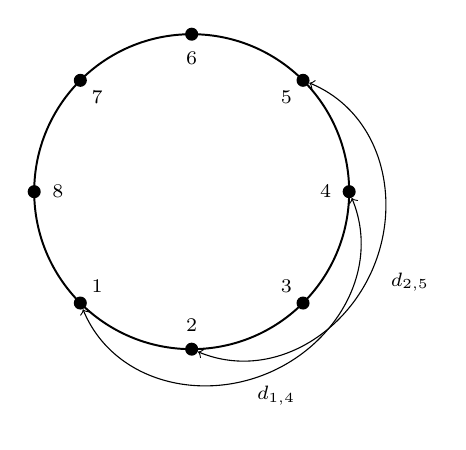
\begin{tikzpicture}[font=\scriptsize, node/.style={circle,thick,draw},
		l_2/.style={line width =0.25mm},
		scale=1, transform shape]
		% equidistant points and arc
		\foreach \x [count=\p] in {0,...,7} {
			\node[shape=circle,fill=black, scale=0.5] (\p) at (\x*45-135:2) {};
		};
		\foreach \x [count=\p] in {0,...,7} {
			\draw (225 + \x*45:1.7) node {\p};
			%				\draw (-30-\x*60:2.4) node {$\bar{\p}$};
		}; 
		\draw[l_2] (4) arc (0:360:2);
		\node (a) at (-22.5:3) {$d_{2, 5}$};
		\draw[<->] (2)  to [out=-22.5,in=-112.5] (-22.5:2.5) to [out=67.5,in=-22.5](5);
		\node (b) at (-67.5:2.8) {$d_{1, 4}$};
		\draw[<->] (1)  to [out=-67.5,in=-157.5] (-67.5:2.5) to [out=22.5,in=-67.5] (4);
		
		\node (bottom) at (0, -2.8) {};
		%		\draw[dashed] (1) -- (3) -- (5) -- (1);
		% axes
		%		\draw [dotted, gray] (-2.6,0) -- (2.6,0);
		%		\draw [dotted, gray] (0,-2.15) -- (0,2.15);
		\end{tikzpicture}
		\subcaption{$d_{1, 4}$ and $d_{2, 5}$ are crossing.}
	\end{minipage}
	%	\hspace{1cm}
	\begin{minipage}[t]{.4\textwidth}
		\begin{tikzpicture}[font=\scriptsize, node/.style={circle,thick,draw},
		l1_green/.style={thick, green!80!black},
		l1_red/.style={thick, blue!80!white},
		l_2/.style={},
		l_3/.style={line width =0.25mm},
		scale=1, transform shape]
		\draw[l_3] (2, 0) arc (0:360:2);
		
		\draw[l1_green] (5) arc (45:90:2);
		\draw[l1_green] (8) arc (180:270:2);
		\draw[l1_red] (4) arc (0:45:2);
		% equidistant points
		\foreach \x [count=\p] in {0,...,7} {
			\node[shape=circle,fill=black, scale=0.5] (\p) at (\x*45-135:2) {};
		};
		% labels
		\foreach \x [count=\p] in {0,...,7} {
			\draw (225 + \x*45:1.7) node {\p};
			%				\draw (-30-\x*60:2.4) node {$\bar{\p}$};
		};
		
		\node (a) at (10:2.9) {$d_{2, 5}$};
		\draw[l_2, <->] (2)  to [out=-22.5,in=-112.5] (-22.5:2.8) to [out=67.5,in=-22.5](5);
		
		\node (b) at (-15:2.46) {$d_{2, 4}$};
		\draw[l_2,<->] (2)  to [out=-15,in=-135] (-45:2.25) to [out=45,in=-75] (4);
		
		\node (c) at (135:2.7) {$d_{6, 8}$};
		\draw[l_2, <->] (6)  to [out=157.5,in=45] (135:2.4) to [out=-135,in=112.5] (8);
		
		\node (bottom) at (0, -2.8) {};
		%		\draw[dashed] (1) -- (3) -- (5) -- (1);
		% axes
		%		\draw [dotted, gray] (-2.6,0) -- (2.6,0);
		%		\draw [dotted, gray] (0,-2.15) -- (0,2.15);
		\end{tikzpicture}
		\subcaption{$d_{2,4}$ and $d_{2, 5}$ and $d_{6, 8}$ are parallel.}
	\end{minipage}
	\caption{Examples of crossing and parallel demands.
		In (b), the green edges lie in between $d_{2, 5}$ and $d_{2, 8}$.
		The blue edge is the only edge in between $d_{2, 4}$ and $d_{2, 5}$.}
	\label{fig:parallel-demands}
\end{figure}
	
	Parallel demands can occur in three types of configurations, which can be seen in \cref{fig:parallel-demands}.
	We distinguish the three cases:
	\begin{enumerate}[align=left]
		\item[\textbf{Cases 1 and 2:} $[i, j) \subset [g, h)$ or $[g, h) \subset [i,j)$]{\mbox{}\\
			We assume $[i, j) \subset [g, h)$; the other case is reasoned analogously.
			Then the rerouting of the traffic results $\phi'$ given by
			\begin{align}
				\phi'(i, j) = 1 \ ,\quad
				\phi'(g, h) = \frac{\beta - \alpha}{d_{gh}}
			\end{align}
			and $\phi'(u, v) = \phi^\ast(u, v)$ for all other demands $d_{uv}$.
			For all $1 \leq m \leq n$, the new link loads are given by
			\begin{equation}
				L_m' = L_m^\ast + \alpha (\dOne_{\{m \in [i, j)\}} - \dOne_{\{m \notin [i, j)\}} + 
				\dOne_{\{m \notin [g, h)\}} - \dOne_{\{m \in [g, h)\}}) \ ,
			\end{equation}
			$\dOne$ being the indicator function.
			If $m \in [i, j)$, then $m \in [g, h)$ and $L_m' = L_m^\ast$.
			If $m \notin [i, j)$, then  $L_m' \leq L_m^\ast$.
		}
		\item[\textbf{Case 3:} $[i, j) \cap [g, h) = \emptyset$]{\mbox{}\\
			In this case the routing $\phi'$ is given by
			\Todo{Explain where this comes from}
			\begin{align}
				\phi'(i, j) = 1 \ ,\quad
				\phi'(g, h) = 1 - \frac{\beta - \alpha}{d_{gh}}
			\end{align}
			and $\phi'(u, v) = \phi^\ast(u, v)$ for all other demands $d_{uv}$.
			The new link loads are given by
			\begin{equation}
				L_m' = L_m^\ast + \alpha (\dOne_{\{m \in [i, j)\}} - \dOne_{\{m \notin [i, j)\}} + 
				\dOne_{\{m \in [g, h)\}} - \dOne_{\{m \notin [g, h)\}}) \ .
			\end{equation}
			Similar to the cases 1 and 2, we get $L_m' \leq L_m^\ast$, as we assumed that $[i, j) \cap [g, h) = \emptyset$.
		}
	\end{enumerate}
	In total, the routing $\phi'$ has link loads $L_m' \leq L_m^\ast$ for all $1 \leq m \leq n$ and $L_k' < L_k^\ast$.
	This contradicts the minimality of $\phi^\ast$.
\end{proof}

We can imagine a cut $\{i, j\}$ as a chord connecting the link $\{i, i+1\}$ with the link $\{j, j+1\}$ and can therefore also use the same terms to describe their properties as for demands, such as \emph{crossing} and \emph{parallel}.

\begin{definition}
	The \emph{demand across the cut} $\{g, h\}$ with $g \neq h$ is the sum of demands with endpoints on both sides of the cut:
	\begin{equation}
		D_{gh} \coloneqq \sum_{d_{ij} \in \{d_{ij}\ |\ \abs{[i, j) \cap (g, h]} = 1\}} \ .
	\end{equation}
	For the degenerate cuts $\{g, g\}$ we define $D_{gg} \coloneqq 2 C_g$.
\end{definition}

\begin{definition}[Cut Condition]
	An cut $\{g, h\}$ is said to satisfy the \emph{cut condition} if
	\begin{equation}
		D_{gh} \leq C_g + C_h \ .
	\end{equation}
	An instance $I$ satisfies the cut condition if each cut does.
	$C_g + C_h - D_{gh}$ is called the \emph{slack} of the cut $\{g, h\}$.
\end{definition}

In an instance of \RRL, is there is a cut $\{g, h\}$ which violates the cut condition, the instance is not solvable:
The links $\{g, g+1\}$ and $\{h, h+1\}$ pose a bottleneck to the demands that cross the cut and hinder every demand from being satisfied.


\begin{theorem}
	\label{theo:cut-condition}
	Let $I$ be an instance of \RRL.
	If all cuts in $I$ satisfy the cut condition, $I$ is solvable.
\end{theorem}
For the proof, we will need the following lemma:
\begin{lemma}
	\label{lemma:parallel-diagonal-cuts}
	Let $\{g, h\}$, $\{g', h'\}$ be two parallel cuts.
	Then every demand crosses as many of the cuts $\{g, h\}$, $\{g', h'\}$ as it crosses cuts $\{g, g'\}, \{h, h'\}$
\end{lemma}
\begin{proof}
	By distinction of cases.
\end{proof}
\begin{proof}[Proof of \cref{theo:cut-condition}]
	We conduct the proof by assuming there are instances that satisfy the cut condition, but are not solvable.
	Let $I$ be the smallest of these instances in terms of ring size $n$ and the number of non-zero demands.
	
	We now construct a new non-solvable instance $I'$ with one less non-zero demand and show that this instance still satisfies the cut condition.
	This will contradict the minimality of $I$, implying that no such instance exists.
	
	For that, pick any non-zero demand $d_{ij}$ with $j - i \geq 2$.
	
	If none exists, all non-zero demands in $I$ must be of the form $d_{i, i+1}$.
	Pick any such demand $d_{i, i+1}$ of which there must be at least one, as otherwise any routing solves $I$.
	Then, renumber the nodes and links by "rotating" such that $d_{i, i+1}$ corresponds to $d_{1, n}$ in the renumbered instance, which still satisfies minimality in the above sense.
	Continue with the new instance in which it is possible to pick a non-zero demand $d_{ij}$ with $j - i \geq 2$.
	
	Hence, we have a non-zero demand with $j - i \geq 2$. 
	Let $\{g, h\}$ be a cut with minimal slack $M$ along the front route of $d_{ij}$, that is a cut $\{g, h\}$ with $i \leq g < h < j$ that minimizes $C_g + C_h - D_{gh}$.
	We construct a new instance $I'$ by pretending to route $\frac{M}{2}$ traffic of $d_{ij}$ along the front route and the remaining $d_{ij} - \frac{M}{2}$ along the back route.
	We decrease the capacities of the new instance accordingly, that is $C_k' = C_k - \frac{M}{2}$ for links on the front route and $C_k' = C_k - (d_{ij} - \frac{M}{2})$ on the back route.
	The demands remain the same with the exception of $d_{ij}$, which is now 0.
	It is easy to see that the new instance is still not solvable; otherwise we could use any feasible routing for $I'$ to construct a solution to $I$.
	
	
	By construction, all cuts $\{s, t\}$ in $I'$ that lie on the front route of $d_{ij}$ still satisfy the cut condition:
	\begin{equation}
		D_{st}' = D_{st} \leq C_{s} + C_{t} - M = (C_{s} - \frac{M}{2}) + (C_{t} - \frac{M}{2}) \stackrel{\mathrm{Def.}}{=} C_{s}' + C_{t}' \ .
	\end{equation}
	The first equality follows from the fact that $d_{ij}$ does not contribute to $D_{st}$ and $D_{st}'$, the inequality from the choice of $M$.
	Similarly, all cuts $\{s, t\}$ that $d_{ij}$ crosses satisfy the cut condition.
	Assume $s \notin [i, j), t \in [i, j)$ without loss of generality, then the following holds true:
	\begin{equation}
		D_{st}' = D_{st} - d_{ij} \leq C_s + C_t - d_{ij} = (C_s - (d_{ij} - \frac{M}{2})) + (C_t - \frac{M}{2}) \stackrel{\mathrm{Def.}}{=} C_s' + C_t' \ .
	\end{equation}
	Here, the first equality results from $d_{ij}$ no longer contribution to the demand of cuts which it crosses.
	The inequality is simply the cut condition in $I$.
	
	Now, pick any cut $\{s, t\}$ which lies on the back route of $d_{ij}$ and assume that it does not satisfy the cut condition.
	This means that
	\begin{equation}
		D_{st} = D_{st}' > C_s' + C_h' = C_s + C_h - 2(d_{ij} - \frac{M}{2}) \ .
	\end{equation}
	or equivalently $D_{st} +  2(d_{ij} - \frac{M}{2}) > C_s + C_h
	This and \cref{lemma:parallel-diagonal-cuts} implies that
	\begin{align}
		D_{sg} + D_{th} \geq D_{st} + D_
	\end{align}
	
	
	We now show that $I'$ still satisfies the cut condition by contradiction.
	Thus, assume there is a cut $\{g', h'\}$ in $I'$ which does ot satisfy the cut condition.


	
\end{proof}

\begin{figure}[ht]
	\begin{algorithm}[H]
		\KwData{Ring size $n \in \N$, demands $d_{ij}$, $1 \leq i < j \leq n$.}
		$M = \max_{1 \leq i < j \leq n} D_{ij}$\;
		\For{$i=1, \ldots, n$}{
			$C_i = \max \left(\max_{1 \leq j < i}(D_{ji} - C_j), \max_{i < j \leq n}(D_{ij} - \frac{M}{2})\right)$ \;
		}
		\While{$\exists \text{parallel demands } d_{ij}, d_{gh}$}{
			Choose link $\{k, k+1\}$ that lies in between $d_{ij}$ and $d_{gh}$\;
			$\{k, l\} \coloneqq \min_{l \neq k} C_k + C_l - D_{kl}$\;
			Assume $d_{ij}$ crosses $\{k, l\}$\;
			Route $d_{gh}$ such that it misses $\{k, l\}$\;
			// Wollen cut constraint als Invariante idealerweise
		}
%		\While{not converged}{
%			\For{$i=1, \ldots, k$}{
%				Sample batch of $B$ samples $z_1, \ldots, z_B$ from $p_z$\;
%				Sample batch $x_{i_1}, \ldots, x_{i_B}$ from the training data\;
%				Compute the stochastic gradient 
%				$$\nabla_{\theta_D} \frac{1}{B} \sum_{j=1}^{B} \left( \ln D(x_{i_j}) + \ln(1 - D(G(z_j))) \right);$$
%				Update $\theta_D$ by ascending the gradient according to the learning rule $R$\;
%			}
%			Sample batch of $B$ samples $z_1, \ldots, z_B$ from $p_z$\;
%			Compute the stochastic gradient
%			$$\nabla_{\theta_G} \frac{1}{B} \sum_{j=1}^{B} -\ln(D(G(z_j)));$$
%			Update $\theta_G$ by descending the gradient according to the learning rule $R$\;
%		}
		\Return{$\phi$}
		\caption{Algorithm for \RRL}
		\label{algo:rrl}
	\end{algorithm}
\end{figure}

\begin{theorem}
	\label{theo:rll-algo-correct}
	Let $I$ be an instance of size $n$ of \RRL that satisfies the cut condition.
	Then \cref{algo:rll} computes a minimal solution of $I$ in $\cO(?)$ time using $\cO(?)$ space.
\end{theorem}
\begin{proof}
	TBD
\end{proof}

\begin{lemma}
	At the end of \cref{algo:rll} at most $\lfloor\frac{n}{2}\rfloor$ demands are split.
\end{lemma}
\begin{proof}
	Let $\phi^\ast$ be the minimal routing that results from the execution of \cref{algo:rll}.
	Furthermore, let $S \coloneqq \{(i, j)\ |\ d_{ij}\ \text{is split by}\ \phi^\ast \}$ and $(i, j), (g, h) \in S$.
	If the demands $d_{ij}$ and $d_{gh}$ were parallel, there would be a link $\{k, k+1\}$ that carries traffic from both demands, as they both are split.
	However, it follows from the minimality of $\phi^\ast$ and \cref{theo:parallel-demands-non-crossing} that this cannot be the case, which implies that $d_{ij}$ and $d_{gh}$ are crossing.
	This can, by definition, only occur if $i, j, g, h$ are mutually distinct.
	
	This implies that every $1 \leq i \leq n$ can occur in at most one tuple in $S$.
	As the tuples in $S$ each consist of two elements, there can be at most $\lfloor\frac{n}{2}\rfloor$ such tuples.
\end{proof}